\documentclass[]{beamer}
% Class options include: notes, notesonly, handout, trans,
%                        hidesubsections, shadesubsections,
%                        inrow, blue, red, grey, brown

% Theme for beamer presentation.
\usepackage{beamerthemesplit} 
% Other themes include: beamerthemebars, beamerthemelined, 
%                       beamerthemetree, beamerthemetreebars  

\title{Orbital Optimization in VB}    % Enter your title between curly braces
\author{Jeroen Engelberts}            % Enter your name between curly braces
%\institute{SURFsara}                 % Enter your institute name between curly braces
\date{\today}                         % Enter the date or \today between curly braces

\begin{document}

% Creates title page of slide show using above information
\begin{frame}
  \titlepage
\end{frame}

\section[Outline]{}

% Creates table of contents slide incorporating
% all \section and \subsection commands
\begin{frame}
  \tableofcontents
\end{frame}


\section{Valence Bond Theory}
\subsection{Introduction}
\begin{frame}
  \frametitle{Goal}   % Insert frame title between curly braces
  Analyze the orbital optimization process in VB and look for possibilities to improve the performance, \textit{i.e.} decrease the computation time.
\end{frame}

\subsection{Valence Bond Wave Functions}
\begin{frame}
  \frametitle{Structures, Determinants \& Orbitals}
  \begin{equation*}
    \Psi = \sum_{i} C_i \Phi_i
  \end{equation*}

  \begin{equation*}
    \Phi = \sum_{i} \alpha_i \Delta_i
  \end{equation*}

  \begin{equation*}
    \Delta = |ijkl \cdots n|
  \end{equation*}

  \begin{equation*}
    i = \sum_{n} c_n \chi_n
  \end{equation*}
\end{frame}

\begin{frame}
  \frametitle{Single Structure Wave Function}
  \begin{center}
  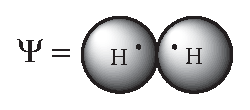
\includegraphics{../figures/heitler.eps}  
  \end{center}
  \begin{equation*}
    \Psi = |1s_{A}\overline{1s_{B}}| - |\overline{1s_{A}}1s_{B}|
  \end{equation*}
\end{frame}

\subsection{Simple slide with three points shown in succession}

\begin{frame}
  \frametitle{Simple slide with three points shown in succession}   % Insert frame title between curly braces

  \begin{itemize}
  \item<1-> Point 1 (Click ``Next Page'' to see Point 2) % Use Next Page to go to Point 2
  \item<2-> Point 2  % Use Next Page to go to Point 3
  \item<3-> Point 3
  \end{itemize}
\end{frame}

\section{Slide with two columns: items and a graphic}
\begin{frame}
  \frametitle{Slide with two columns: items and a graphic}   % Insert frame title between curly braces
  \begin{columns}[c]
  \column{2in}  % slides are 3in high by 5in wide
  \begin{itemize}
  \item<1-> First item
  \item<2-> Second item
  \item<3-> ...
  \end{itemize}
  \column{2in}
  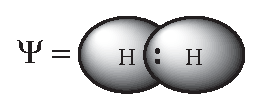
\includegraphics[height=0.5in]{../figures/coulson.eps}
  \end{columns}
\end{frame}

\end{document}
